\documentclass[]{article}
\usepackage[utf8]{inputenc}
\usepackage[usenames]{color}
\usepackage[spanish]{babel}
\usepackage[latin1]{} % para acentos sin codigo
\usepackage{graphicx} % graficos
\usepackage{float} % para usar [H]
\usepackage{hyperref}
\usepackage[table,xcdraw]{xcolor}
\usepackage{vmargin}

\usepackage[version=3]{mhchem} 

\setpapersize{A4}
\setmargins{3.5cm}      % margen izquierdo
{1.5cm}                 % margen superior
{14cm}                % anchura del texto
{23.42cm}               % altura del texto
{10pt}                  % altura de los encabezados
{1cm}                   % espacio entre el texto y los encabezados
{0pt}                   % altura del pie de página
{2cm}                   % espacio entre el texto y el pie de página



%Parámetros Tablas
\usepackage{booktabs}
\usepackage{multirow, array} % para las tablas


%opening
\title{Resultados\_hw3} 
\author{Diana Melendez Zamora \\ 201218118}
\date{\today}

\begin{document}


\maketitle

\begin{abstract}
Se presentan las gráficas obtenidas al ejecutar los códigos \texttt{Onda.py}, \texttt{Planetas.c} y finalmente \texttt{Plots\_Planetas.py}.
\end{abstract}


\section{Onda $\Phi (t,x,y)$}
\subsection{t = 30}
\begin{figure}[H]
	\centering
	\includegraphics[scale=0.7]{ondaent30.png}
	\caption{{\small Onda en tiempo 30.}}
	\label{fig: ondaent30}
\end{figure}


\subsection{t = 60}
\begin{figure}[H]
	\centering
	\includegraphics[scale=0.7]{ondaent60.png}
	\caption{{\small Onda en tiempo 60.}}
	\label{fig: ondaent60}
\end{figure}



\section{Planetas}
\begin{figure}[H]
	\centering
	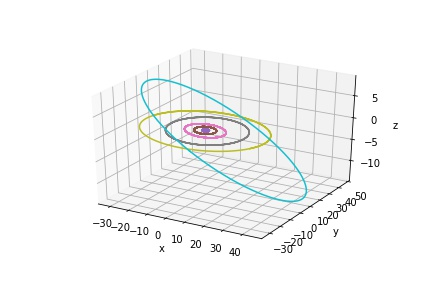
\includegraphics[scale=0.7]{orbitasdelosplanetas.jpg}
	\caption{{\small Orbitas de los planetas.}}
	\label{fig: orbitasdelosplanetas.png}
\end{figure}




\bibliographystyle{APA}
\begin{thebibliography}{9}	
	
	\bibitem{1}
	Repositorio del curso: \\ https://github.com/ComputoCienciasUniandes/MetodosComputacionales/blob/master/notes/

\end{thebibliography}



\end{document}